\documentclass[11pt,aspectratio=43,usenames,dvipsnames]{beamer}
\usepackage[utf8]{inputenc}
\usepackage{amsmath, amsfonts, amssymb, amsthm}
\usepackage[T1]{fontenc}
% mint: code chuck and syntax highlighting
%% outputdir should change according to pdf build directory
\usepackage[outputdir=build,cache=false]{minted}
\usepackage{lmodern}
\usepackage{xcolor}
\usepackage{setspace}
\usepackage{booktabs}
\usepackage{multirow}
\usepackage{graphicx}
\usepackage{fontawesome}

\usepackage[mode=tex]{standalone}
\usepackage{tikz}
\usetikzlibrary{decorations}
\usetikzlibrary{decorations.pathreplacing, intersections}
\usepackage{pgfplots}
\usetikzlibrary{calc,positioning}
\usepgfplotslibrary{fillbetween}
\pgfplotsset{compat=newest, scale only axis, width = 10cm}

% ---------------------------------------------------------------------
% Coordinate extraction
% #1: node name
% #2: output macro name: x coordinate
% #3: output macro name: y coordinate
\newcommand{\Getxycoords}[3]{%
    \pgfplotsextra{%
        % using `\pgfplotspointgetcoordinates' stores the (axis)
        % coordinates in `data point' which then can be called by
        % `\pgfkeysvalueof' or `\pgfkeysgetvalue'
        \pgfplotspointgetcoordinates{(#1)}%
        % `\global' (a TeX macro and not a TikZ/PGFPlots one) allows to
        % store the values globally
         \global\pgfkeysgetvalue{/data point/x}{#2}%
         \global\pgfkeysgetvalue{/data point/y}{#3}%
     }%
}
% ---------------------------------------------------------------------

\usepackage{ulem}
\usepackage{hyperref}
\usepackage{booktabs}
\usepackage{babel}
\usepackage{makecell}
\usepackage[para,online,flushleft]{threeparttable}
\usepackage{pdfpages}
\usepackage{tcolorbox}
\usepackage{bm}
\usepackage{appendixnumberbeamer}
\usepackage{natbib}
\usepackage{caption}
\captionsetup[figure]{labelformat=empty}% redefines the caption setup of the figures environment in the beamer class.
\usetheme[compress]{Boadilla}
\usecolortheme{default}
\useoutertheme{miniframes}
\usefonttheme[onlymath]{serif}

\newcommand{\jump}[2]{\hyperlink{#1}{\beamerbutton{#2}}}
\newcommand{\extjump}[2]{\href{#1}{\beamerbutton{#2}}}
\newcommand{\orange}[1]{\textcolor{orange}{#1}}
\newcommand{\red}[1]{\textcolor{red}{#1}}
\newcommand{\blue}[1]{\textcolor{blue}{#1}}
\newcommand{\green}[1]{\textcolor{OliveGreen}{#1}}

\renewcommand{\square}{\scalebox{0.7}{$\blacksquare$ \hspace{0.5em}}}
\setbeamertemplate{itemize item}{\raisebox{0.1em}{\scalebox{0.7}{$\blacksquare$}}}
\setbeamertemplate{itemize subitem}[circle]
\setbeamertemplate{itemize subsubitem}{--}
\setbeamercolor{itemize item}{fg=black}
\setbeamercolor{itemize subitem}{fg=black}
\setbeamercolor{itemize subsubitem}{fg=black}
\setbeamercolor{item projected}{bg=darkgray,fg=white}
\definecolor{blue}{rgb}{0.2, 0.2, 0.7}
\setbeamercolor{alerted text}{fg=blue}
\setbeamertemplate{enumerate items}[circle]


\setbeamertemplate{headline}{}

%==========================================
\let\olditemize=\itemize
\let\endolditemize=\enditemize
\renewenvironment{itemize}{\olditemize \itemsep1em}{\endolditemize}
\let\oldenumerate=\enumerate
\let\endoldenumerate=\endenumerate
\renewenvironment{enumerate}{\oldenumerate \itemsep1em}{ \endoldenumerate}

\DeclareMathOperator*{\argmax}{\arg\!\max}
\DeclareMathOperator*{\E}{\mathbb{E}}
\DeclareMathOperator*{\var}{\rm Var}
\DeclareMathOperator*{\cov}{\rm Cov}

\theoremstyle{definition}
\newtheorem{assume}{Assumption}
\newtheorem{lem}{Lemma}
\newtheorem{proposition}{Proposition}
\newtheorem{thm}{Theorem}
\newtheorem{corol}{Corollary}

\AtBeginSection[]{
  \begin{frame}[noframenumbering]
  \vfill
  \centering
  \begin{beamercolorbox}[sep=8pt,center,shadow=true,rounded=true]{title}
    \usebeamerfont{title}\insertsection\par%
  \end{beamercolorbox}
  \vfill
  \end{frame}
}

\begin{document}
    \title[Unit 10]{Unit 10 \\ Banks, Money and the Credit Market }
    \author[Hui-Jun Chen]{Hui-Jun Chen}
    \institute[OSU]{The Ohio State University}
    % \date{\today}
    \date{\today}
    \setbeamertemplate{navigation symbols}{}
    \setstretch{1.2}

%-------------------------------------------------------
{
%	\usebackgroundtemplate{\includegraphics[width=1\paperwidth]{../EveningSky_cropped_edit43_bright.jpg}}
    \begin{frame}
% \vspace{3em}
        \centering
%		{\footnotesize 	ECON 4002 Intermediate Macroeconomic Theory}
        \maketitle
% \vspace{-1.5em}
% \centering
% \includegraphics[width=0.55\linewidth]{Pictures/houses.jpeg}


    \end{frame}
}

% -------------------------------------------
\setbeamertemplate{headline}
{
\setbeamercolor{section in head/foot}{fg=black, bg=white}
\vskip1em \tiny \insertsectionnavigationhorizontal{1\paperwidth}{\hspace{0.50\paperwidth}}{}
}
%------------------------------------------

\section[Intro]{Introduction}
\label{sec:Intro}

\begin{frame}{Introduction \extjump{https://www.core-econ.org/the-economy/book/text/10.html}{Textbook}}
\label{slide:Introduction}
\begin{center}
\begin{quote}
    Economics is a choice between alternatives all the time. Those are the trade-offs.
\end{quote}
\hfill - Paul Samuelson

\begin{itemize}
    \item Food spoils, barrels leak, yet all trades take \alert{time}.
    \item Time is both the friend and the foe: depreciation \& appreciation
    \item \alert{Inter-temporal assets} allow agents to \alert{carry value over time}.
    \item What are inter-temporal assets?
    \begin{table}
        \footnotesize
        \begin{tabular}{r|lllll}
            Examples
                & Money
                & Capital
                & Bond / Debt
                & Social Security
                & Housing
            \\
            \hline
            Value $ \uparrow /\downarrow  $
                & $ \downarrow  $
                & $ \downarrow  $
                & $ \downarrow  $
                & $ \uparrow  $
                & $ \uparrow  $ (?)
            \\
            \hline
            Cause (?)
                & inflates
                & tech
                & default
                & age
                & develop
            \\
        \end{tabular}
        \caption{Examples of Intertemporal Assets}
    \end{table}
\end{itemize}

\end{center}
\end{frame}

\section[Time \faClockO]{Income, Borrowing and Saving}
\label{sec:Income__Borrowing_and_Saving}

\begin{frame}{Money, Income and Wealth}
\label{slide:Money__Income_and_Wealth}
    \begin{itemize}
        \item \textbf{Money}: medium of exchange, allow \alert{transfer} of purchasing power
        \begin{itemize}
            \item Whether a currency is \textbf{trust-worthy} is important
        \end{itemize}
        \item (Flow) \textbf{Income}: amount of money receive for a period of time
        \begin{itemize}
            \item wage bill, market earning, investment, gov transfer
        \end{itemize}
        \item (Stock) \textbf{Wealth}: inter-temporal assets carry values
        \begin{itemize}
            \item buildings, land, machinery, capital goods $ - $ debts $ + $ credit
        \end{itemize}
    \end{itemize}
\end{frame}

\begin{frame}{Other Key Concepts}
\label{slide:Other_Key_Concepts}
    \begin{itemize}
        \item Depreciation / Appreciation: value of stock $ \downarrow / \uparrow  $ over time
        \item Net income $ = $ gross income $ - $ depreciation
        \item Savings: income not consumed
        \item Investment: Expenditure on newly produced capital goods
    \end{itemize}
\end{frame}

\begin{frame}{Inter-temporal Substitution}
\label{slide:Inter_temporal_Substitution}
    \begin{itemize}
        \item As time is here, \alert{current you} and \alert{future you} are sharing for resources
        \item The opportunity cost of \alert{more current goods} is \alert{less future goods}
        \item \textbf{Borrowing} and \textbf{lending} allows resource-sharing across time
        \item The ``price'' for inter-temporal substitution depends on the assets;
        \item In the case of borrowing / lending, we call the ``price'' as \textbf{interest rate}
        \item The position matters: the impact of change in interest rate depends on whether you are \alert{borrower} or \alert{lender}
    \end{itemize}
\end{frame}

\begin{frame}{Borrowing}
\label{slide:Borrowing}
    \begin{columns}
        \begin{column}{0.5\textwidth}
            \only<1>{
            \begin{itemize}
                \item Julia has $ 100 $ endowment in the \alert{future}: Nothing for today. \faFrownO
                \item Julia wants to \alert{borrow} some consumption \alert{today} and promise to repay \alert{tomorrow} with her endowment
                \item How \alert{much} goods could Julia get for today if she commit all her endowment tomorrow?
            \end{itemize}
            }
            \only<2>{
            \begin{itemize}
                \item \textbf{Interest rate ($r$)}: price to bring purchasing power forward in time
                \item current $ \underbrace{\Longrightarrow}_{1+r} $ future
                \item
                \begin{tabular}{cc}
                    today
                        & tomorrow
                    \\
                    1
                        & $ 1+r $
                    \\
                    $ \frac{1}{1+r} $
                        & 1
                    \\
                \end{tabular}
                % \item Slope: $ \frac{1}{1+r} $, since future $ C $ on $ y $-axis and current on $ x $-axis
            \end{itemize}
            }
            \only<3>{
            \begin{itemize}
                \item $ (1+r) $: \textbf{supply-side} tradeoff $ \Rightarrow  $ MRT
                \item Motivation for borrowing \& lending:
                \begin{enumerate}
                    \item \alert{consumption smoothing} (Julia's case)
                    \item \alert{Impatience}
                \end{enumerate}


            \end{itemize}
            }
        \end{column}
        \begin{column}{0.5\textwidth}
            \begin{figure}
                \centering
                \only<1-2>{
                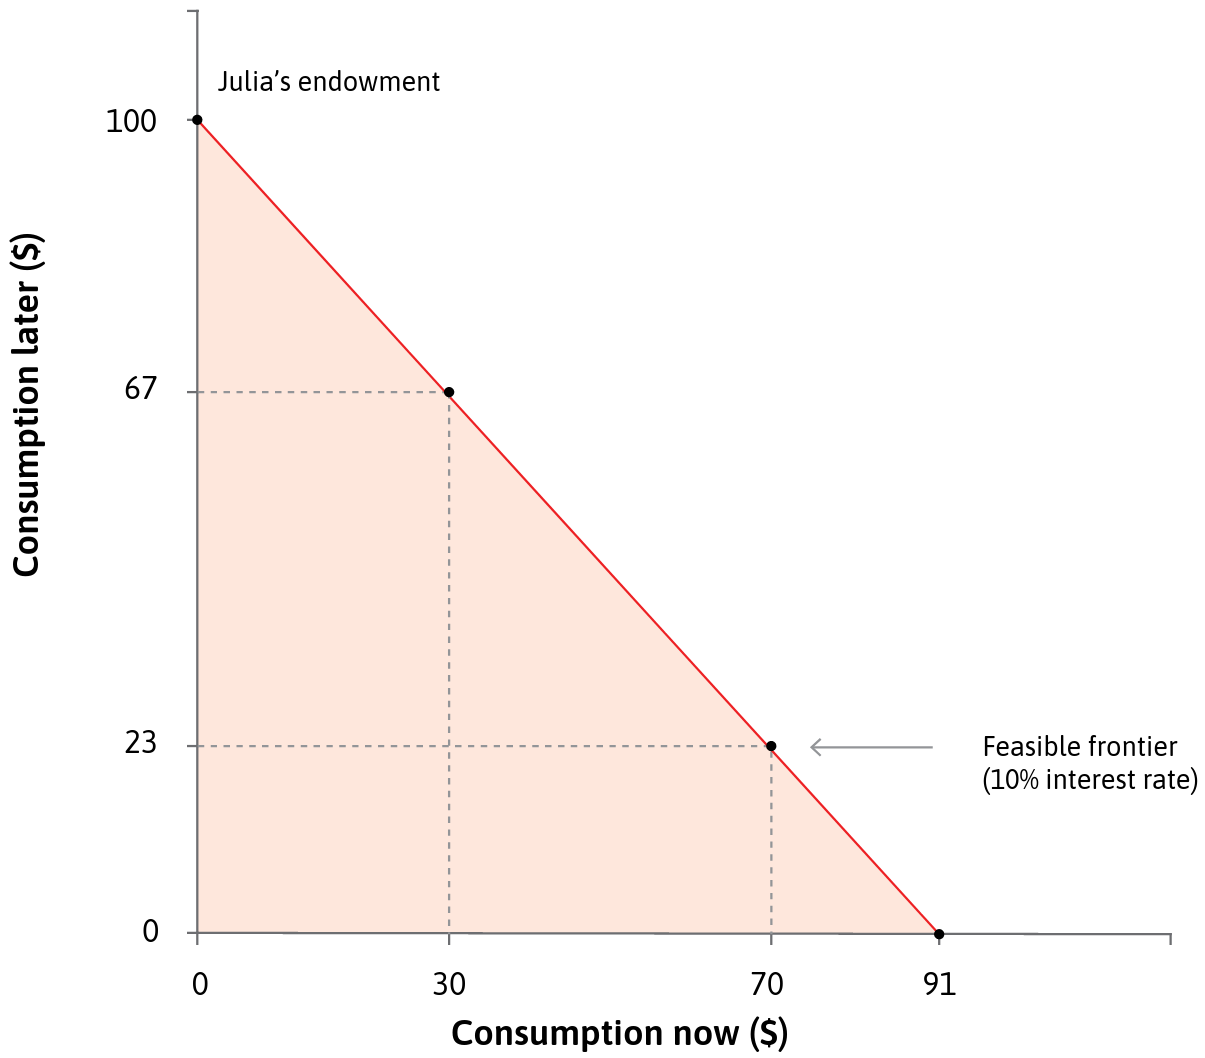
\includegraphics[width=\textwidth]{./figures/Figure1.png}
                }
                \only<3>{
                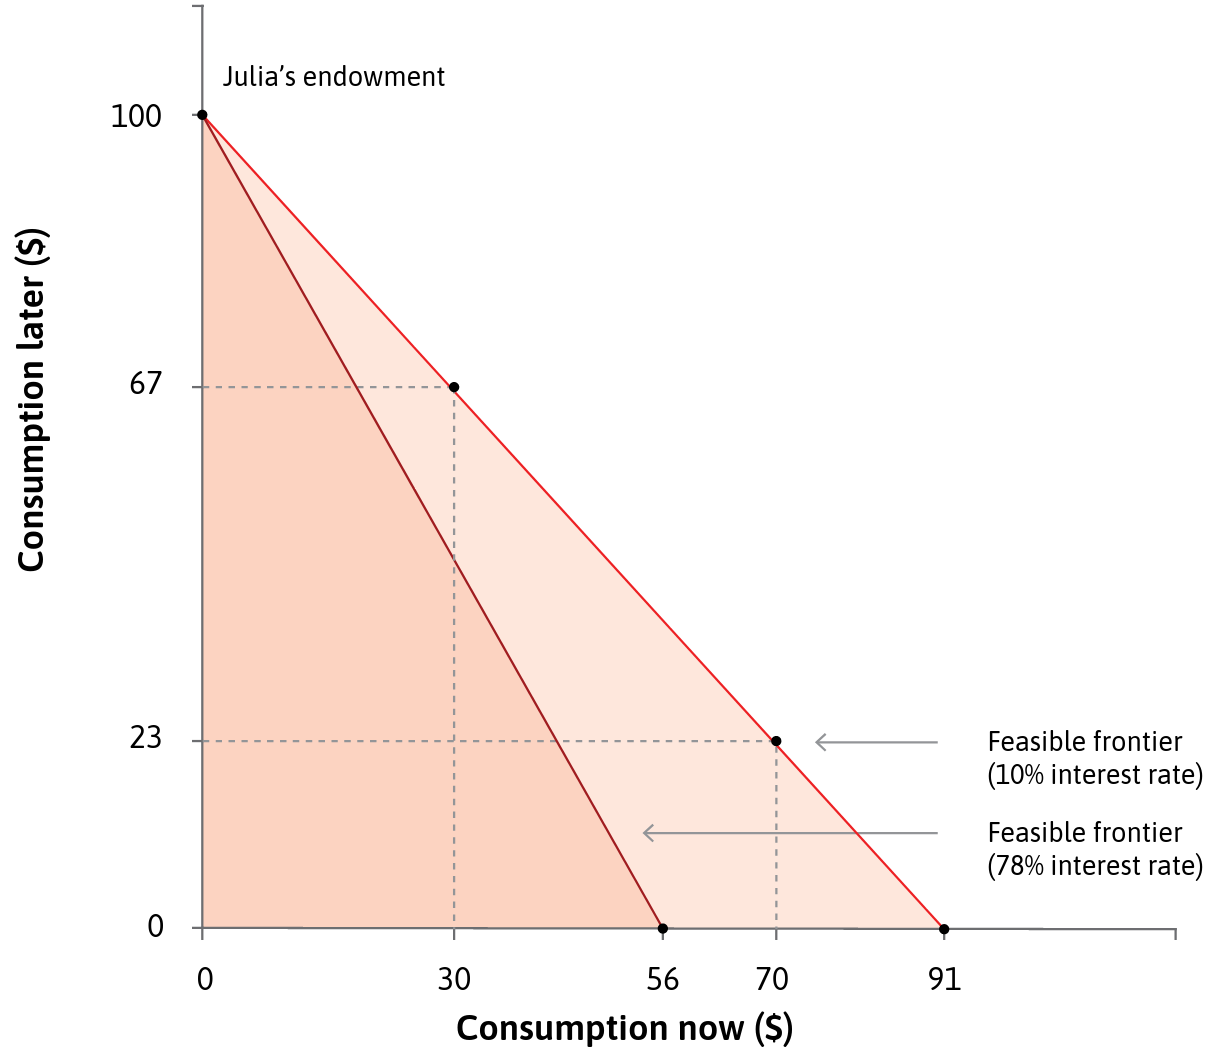
\includegraphics[width=\textwidth]{./figures/Figure2.png}
                }
            \end{figure}
        \end{column}
    \end{columns}
\end{frame}

\begin{frame}{Consumption Smoothing}
\label{slide:Consumption_Smoothing}
    \begin{columns}
        \begin{column}{0.5\textwidth}
            \begin{itemize}
                \item The indifference curve exhibits \textbf{diminishing marginal returns to consumption} in one period.
                \item \alert{Avoid consuming a lot in one period and little in the other.}
                \item \textbf{Discount rate ($ \rho $)}: measure of one's impatience/precautions
            \end{itemize}
        \end{column}
        \begin{column}{0.5\textwidth}
            \begin{figure}
                \centering
                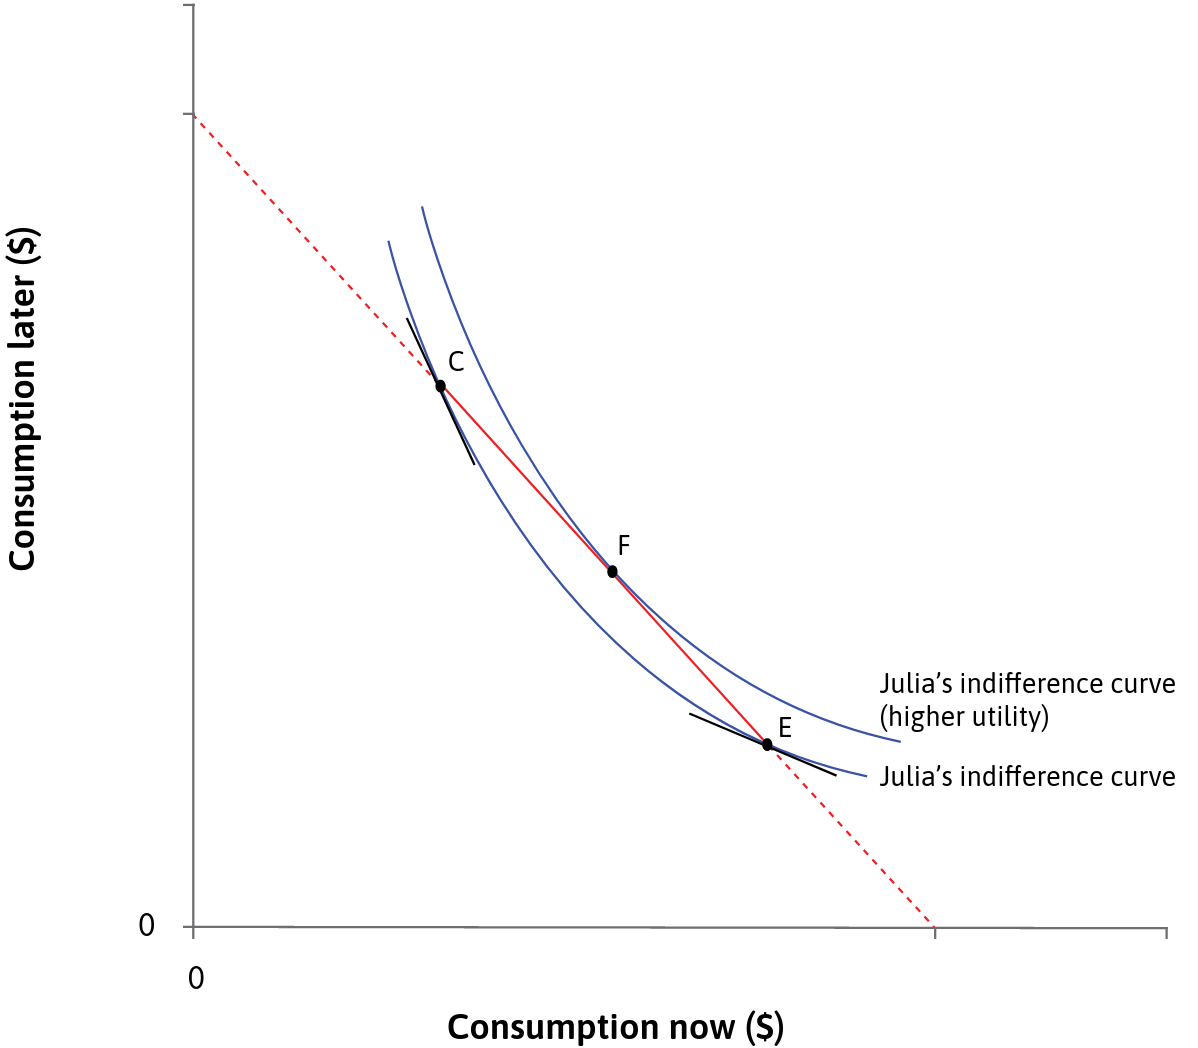
\includegraphics[width=\textwidth]{./figures/Figure3.png}
            \end{figure}

        \end{column}
    \end{columns}
\end{frame}

\begin{frame}{Pure Impatience}
\label{slide:Pure_Impatience}

        \begin{center}
            \textit{How much more do you value a good now than later?}
        \end{center}

        \vspace{1em}

    \begin{itemize}
        \item Consumption smoothing may appear as being impatient.
        \item However, we differentiate it from pure impatience = being impatient as a person.
        \begin{itemize}
            \item \textbf{Myopia} (short-sightedness): People experience the present satisfaction more strongly than the same satisfaction later
            \item \textbf{Prudence}: People know that they may not be around in the future, and so they want to consume now
        \end{itemize}


    \end{itemize}
\end{frame}

\begin{frame}{Optimal Decision-Making for Borrowers}
\label{slide:Optimal_Decision_Making}
    \begin{columns}
        \begin{column}{0.4\textwidth}
            \begin{itemize}
                \only<1>{
                \item In equilibrium $ MRS = MRT $, i.e., $ 1+\rho = 1+r $
                \item At $ 10\% $ interest rate, Julia is happy at point $ E $ (intersection of IC and FF)
                }
                \only<2>{
                \item $ r: 10\% \rightarrow 78\% $, optimal decision: $ E \rightarrow G $ \faFrownO.
                \item Julia hurts since she is \alert{borrowers}:
                \begin{itemize}
                    \item Point $ F $ is when Julia only wants $ 35 $ consumption now under $ 10\% $ of interest rate.
                \end{itemize}
                \item \alert{Income} and \alert{substitution} effects also applies. How?
                }
            \end{itemize}

        \end{column}
        \begin{column}{0.6\textwidth}
            \begin{figure}
                \centering
                \only<1>{
                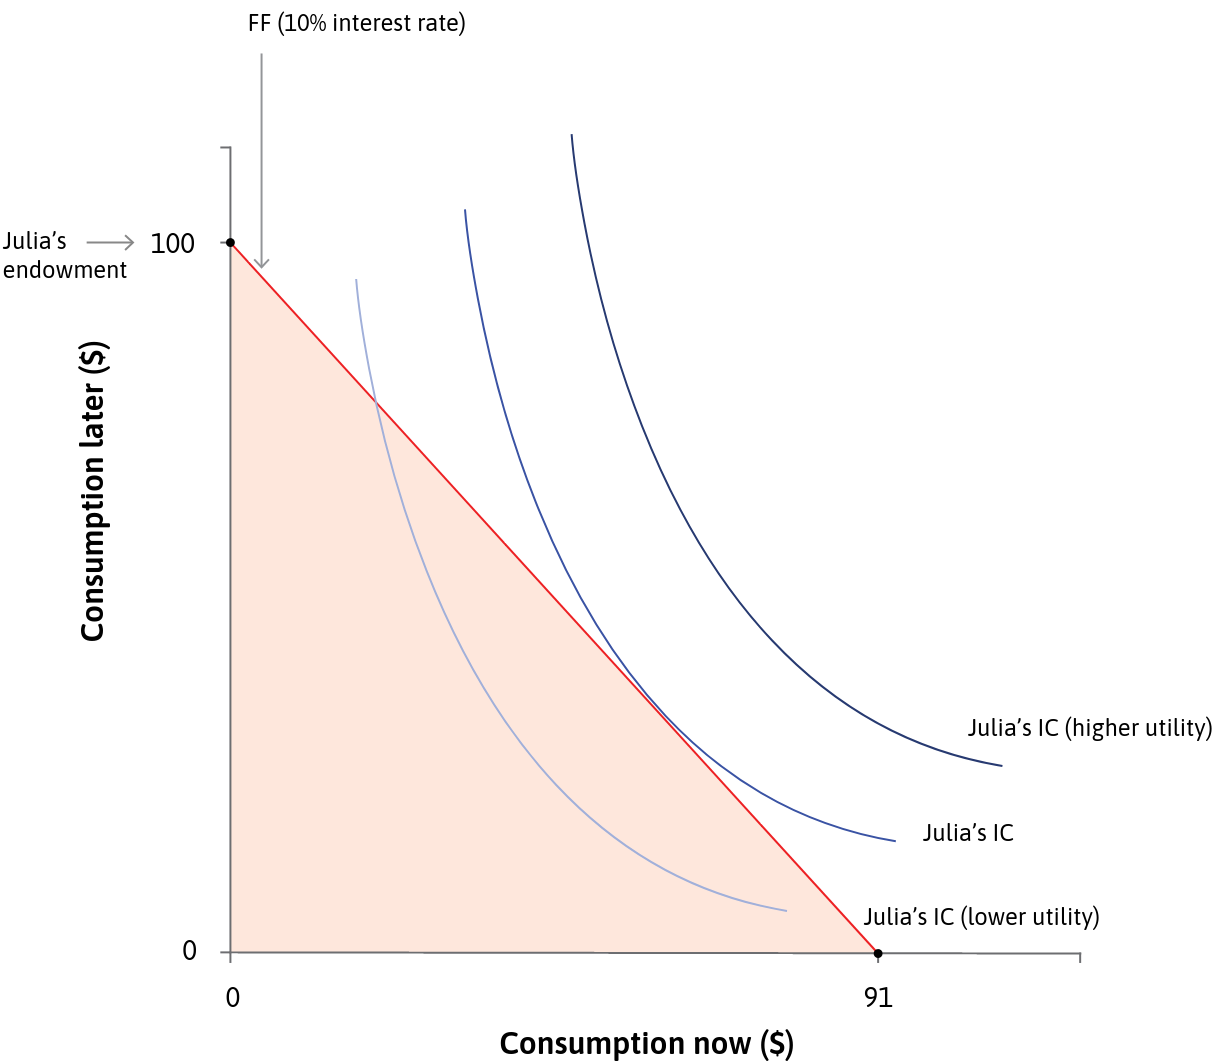
\includegraphics[width=\textwidth]{./figures/Figure5.png}
                }
                \only<2>{
                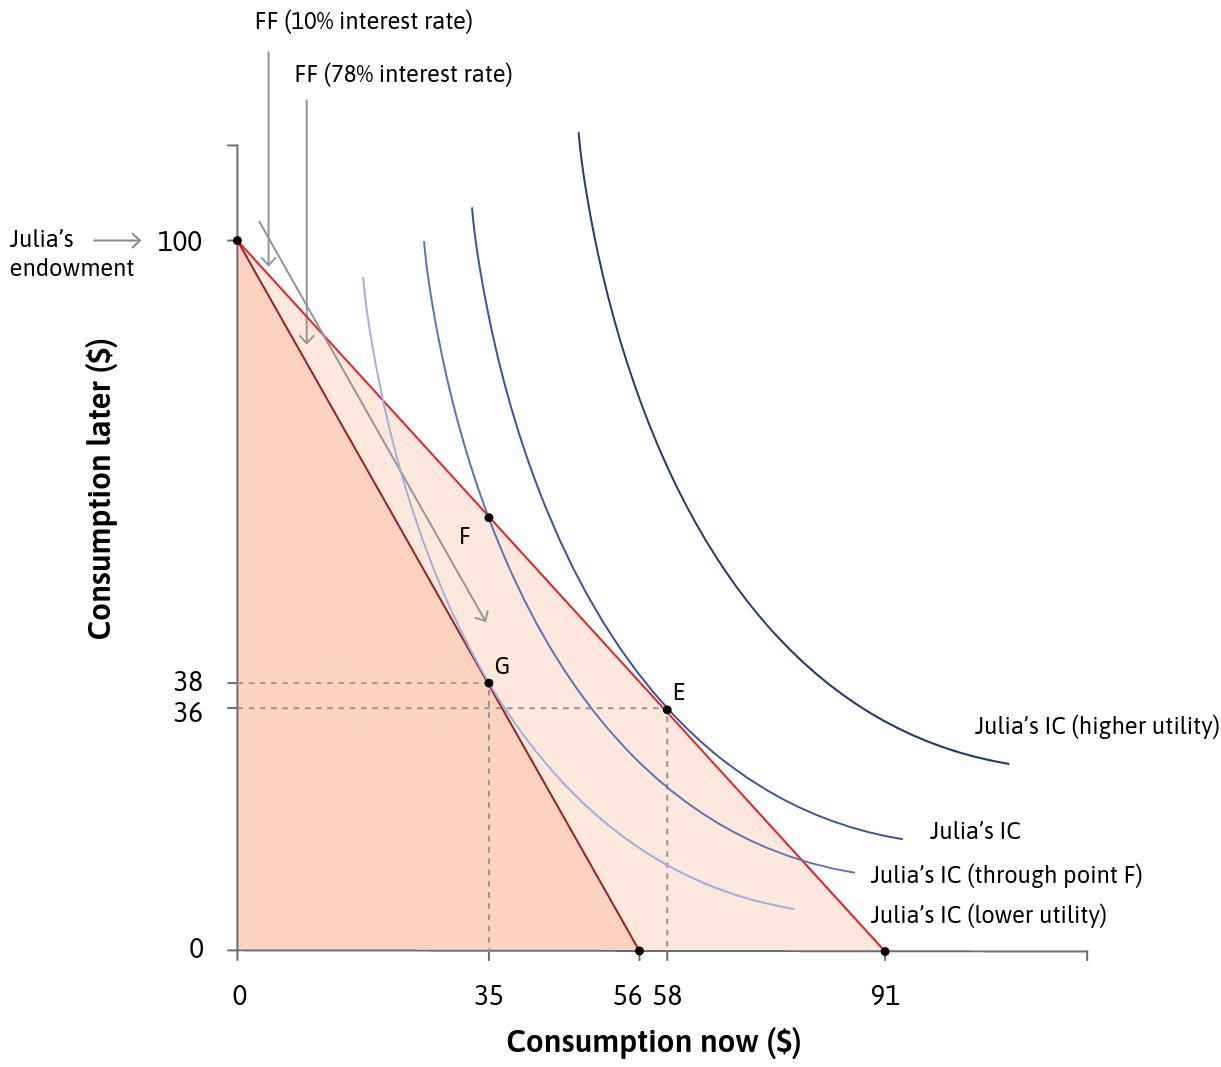
\includegraphics[width=\textwidth]{./figures/Figure6.png}
                }
            \end{figure}

        \end{column}
    \end{columns}


\end{frame}

\begin{frame}{Saving}
\label{slide:Saving}
    \begin{columns}
        \begin{column}{0.4\textwidth}
            \only<1>{
            \begin{itemize}
                \item Marco is a \alert{saver} with $ 100 $ endowment \alert{today}
                \item Macro store his grain: $ 20\% $ of loss
                \item Macro lend to Julia: achieve \alert{medium} utility w/o grain loss
            \end{itemize}
            }
            \only<2>{
            \begin{itemize}
                \item \alert{Reservation indifference curve}: outside option for Marco
                \item What is reservation IC for Julia?
            \end{itemize}
            }
        \end{column}
        \begin{column}{0.6\textwidth}
            \begin{figure}
                \centering
                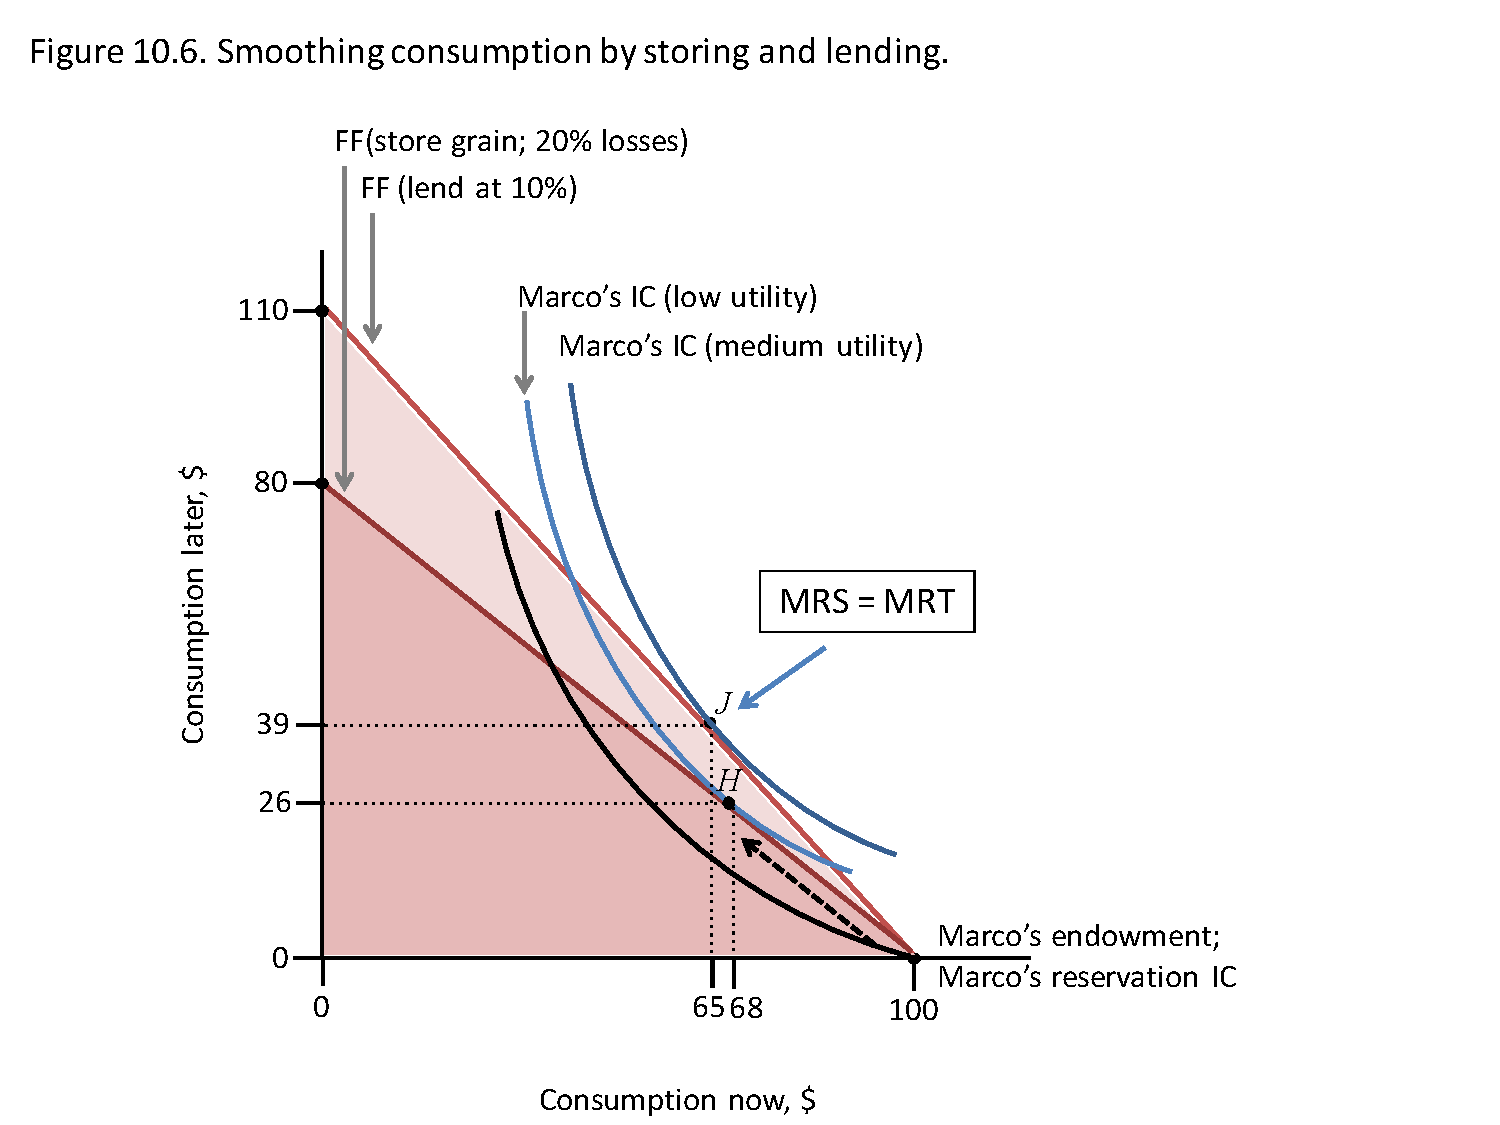
\includegraphics[trim={1.5cm 1.5cm 1.5cm 1.5cm}, clip, width=\textwidth]{./figures/Figure8.pdf}
            \end{figure}

        \end{column}
    \end{columns}

\end{frame}

\begin{frame}{Reservation Indifference Curve}
\label{slide:Reservation_Indifference_Curve}
    \begin{columns}
        \begin{column}{0.4\textwidth}
            \begin{itemize}
                \item Reservation indifference curve: all of the points at which the individual would be just as well off as at the reservation position (endowment).
                \item \alert{Room for trade} is to ensure Marco is happier than reservation IC; o/w Marco is not lending!
            \end{itemize}
        \end{column}
        \begin{column}{0.6\textwidth}
            \begin{figure}
                \centering
                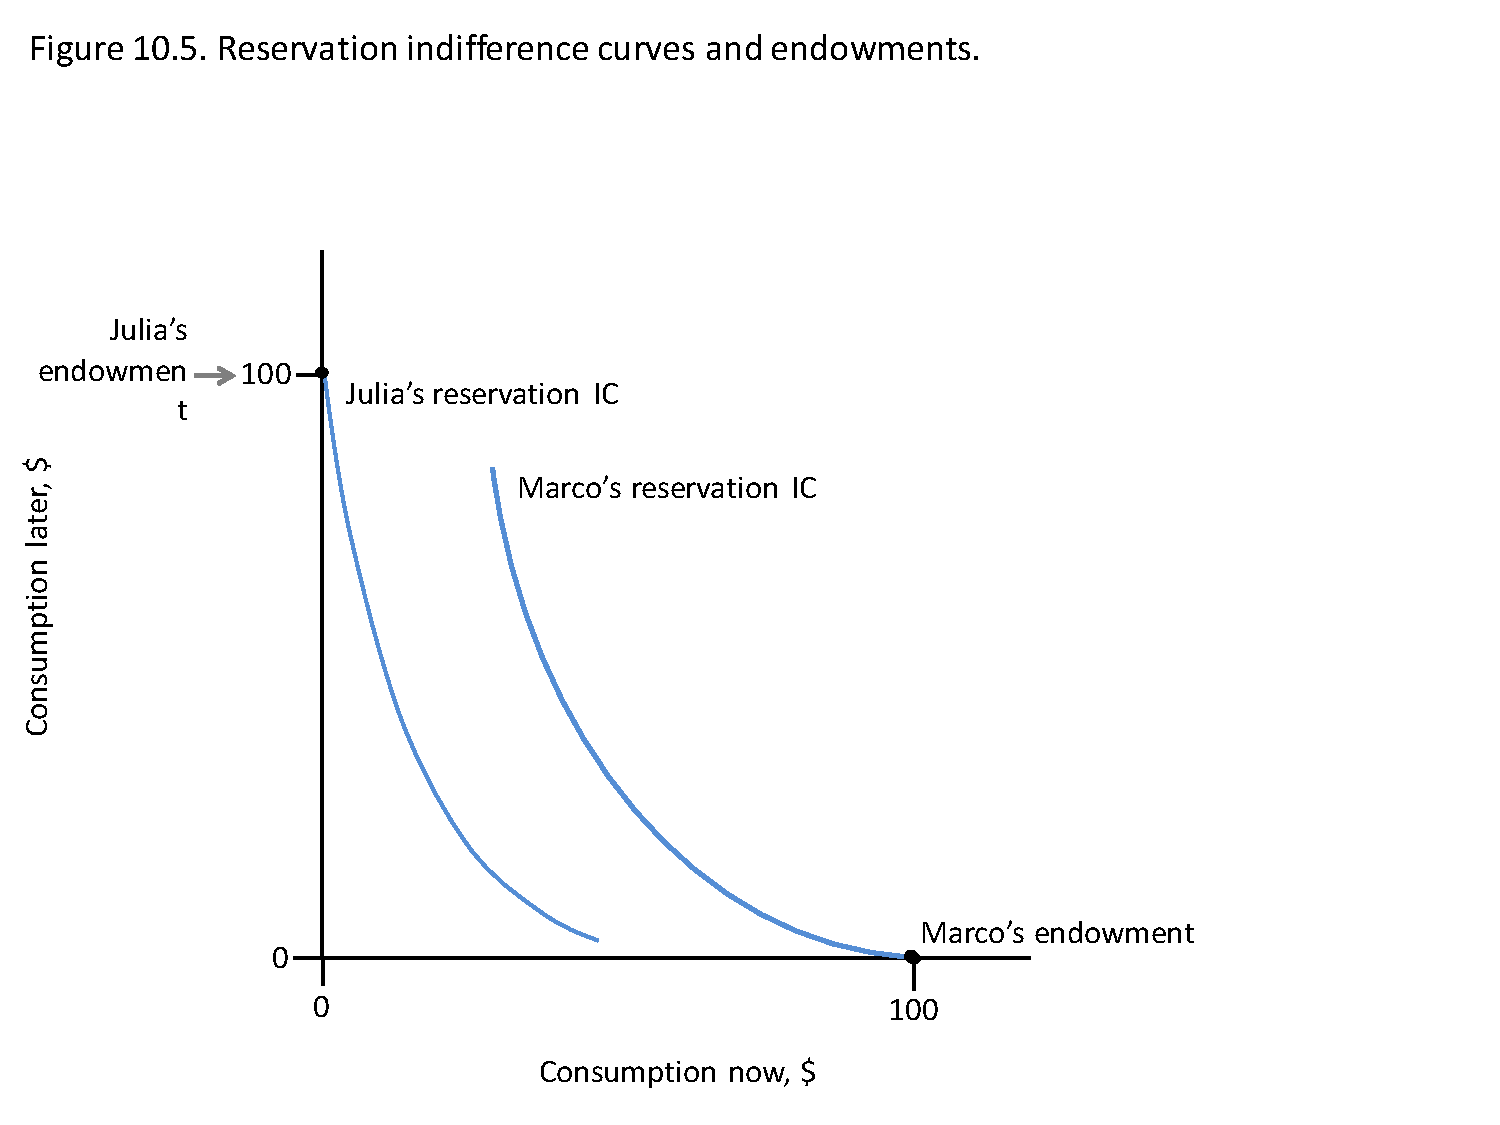
\includegraphics[trim={1.5cm 1.5cm 1.5cm 1.5cm}, clip, width=\textwidth]{./figures/Figure7.pdf}
            \end{figure}

        \end{column}
    \end{columns}

\end{frame}

\section[\faBank \& \faMoney]{Banks and Money}
\label{sec:Banks_and_Money}

\begin{frame}{The Financial System}
\label{slide:The_Financial_System}
    \begin{figure}
        \centering
        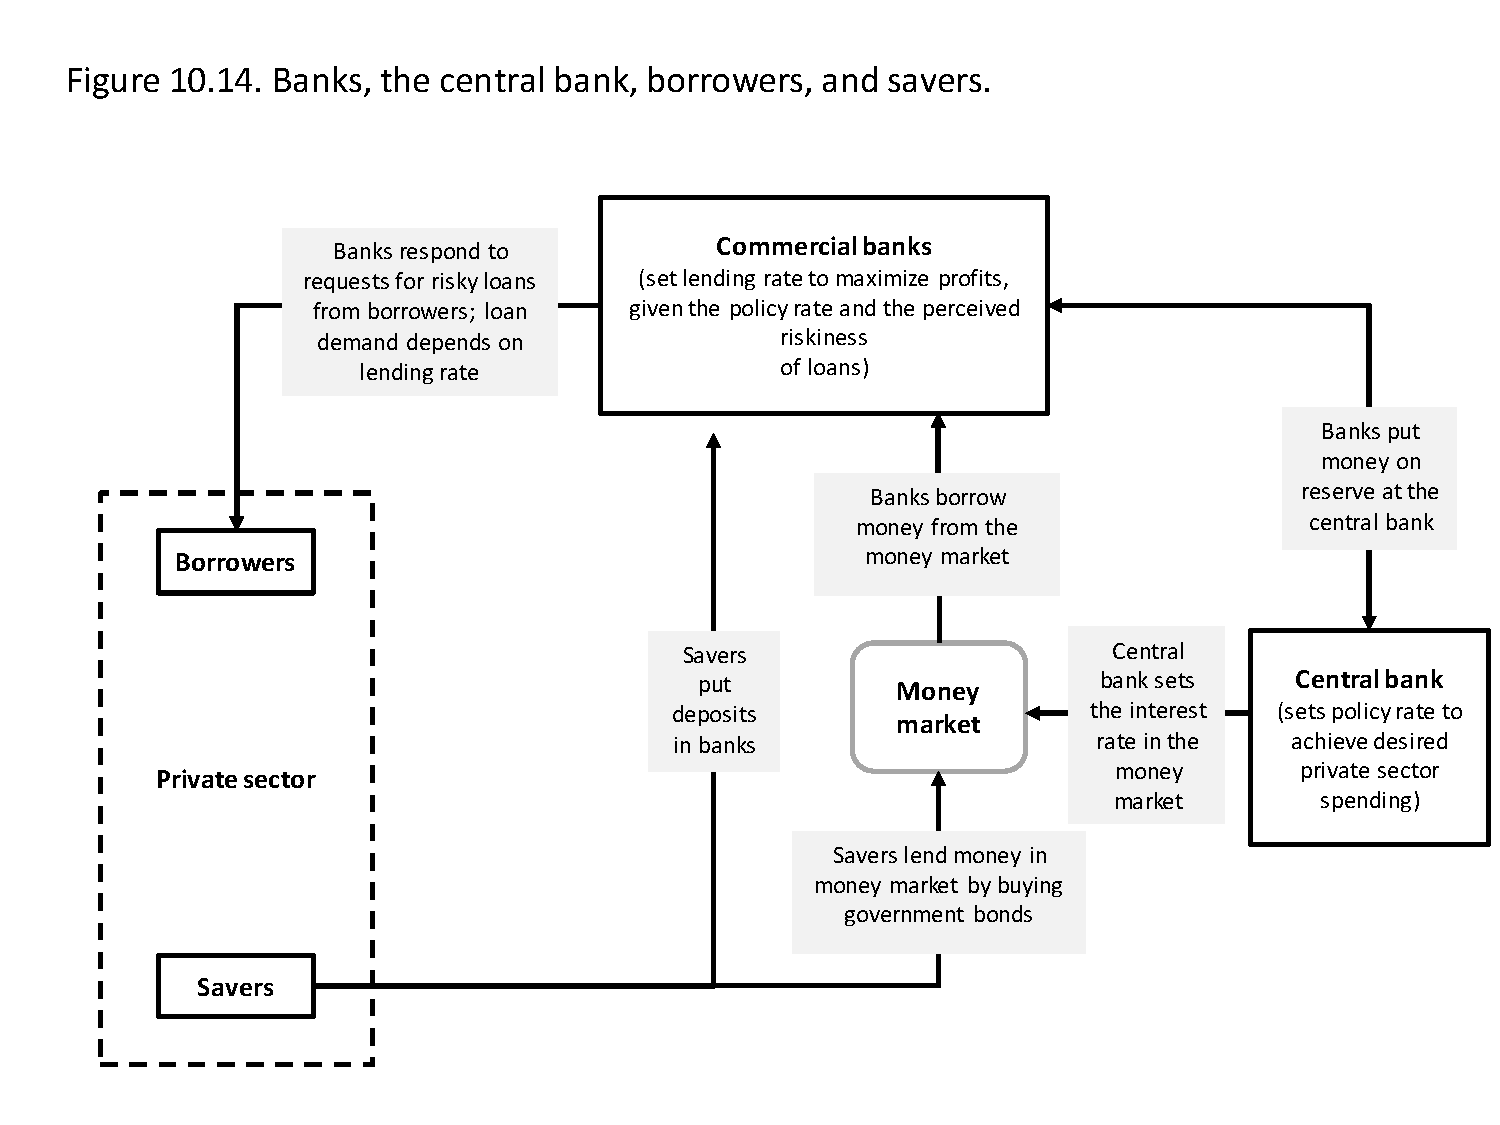
\includegraphics[trim={1cm 1cm 0cm 2.5cm}, clip, width=\textwidth]{./figures/Figure21.pdf}
    \end{figure}

\end{frame}



\begin{frame}{Balance Sheet}
\label{slide:Balance_Sheet}
    \begin{figure}
        \centering
        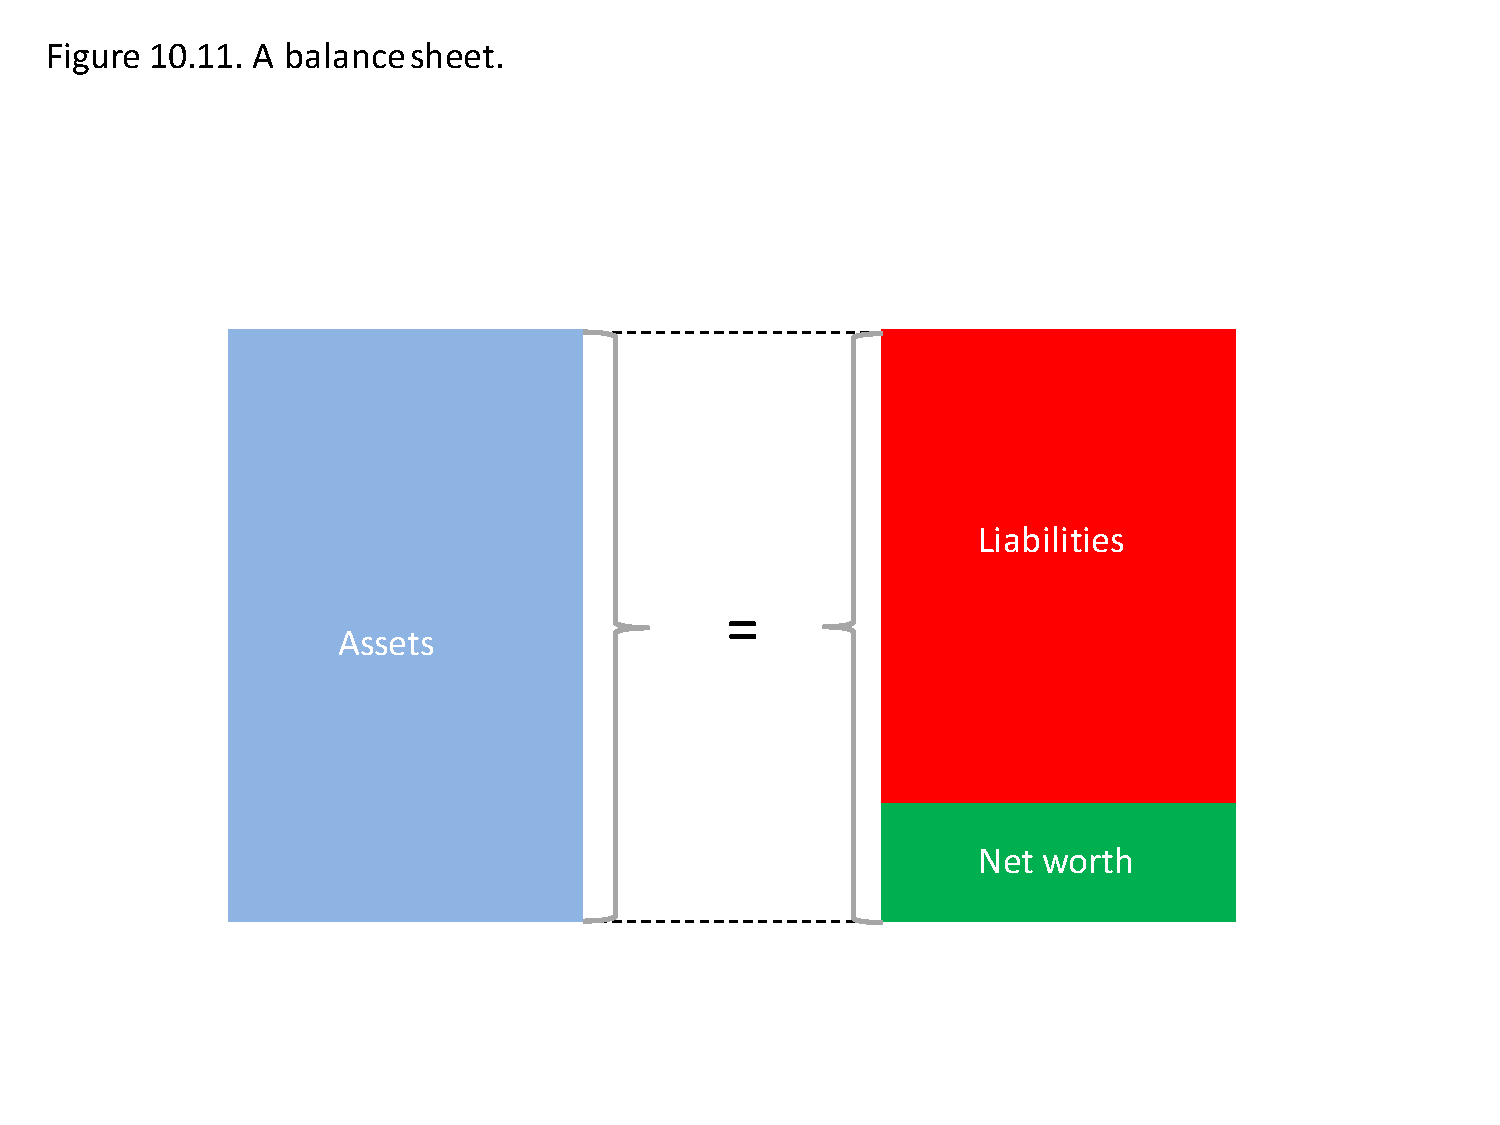
\includegraphics[trim={1.5cm 1.5cm 1.5cm 1.5cm}, clip, width=0.6\textwidth]{./figures/Figure13.pdf}
    \end{figure}
    \begin{itemize}
        \item \alert{Assets}: Anything of value that is owned.
        \item \alert{Liabilities}: Anything of value that is owed.
        \item \alert{Net worth}: assets $ - $ liabilities
    \end{itemize}

\end{frame}

\begin{frame}{Balance Sheet and Wealth}
\label{slide:Balance_Sheet_and_Wealth}
    \begin{columns}
        \begin{column}{0.1\textwidth}
        \end{column}
        \begin{column}{0.9\textwidth}
            \begin{figure}
                \centering
                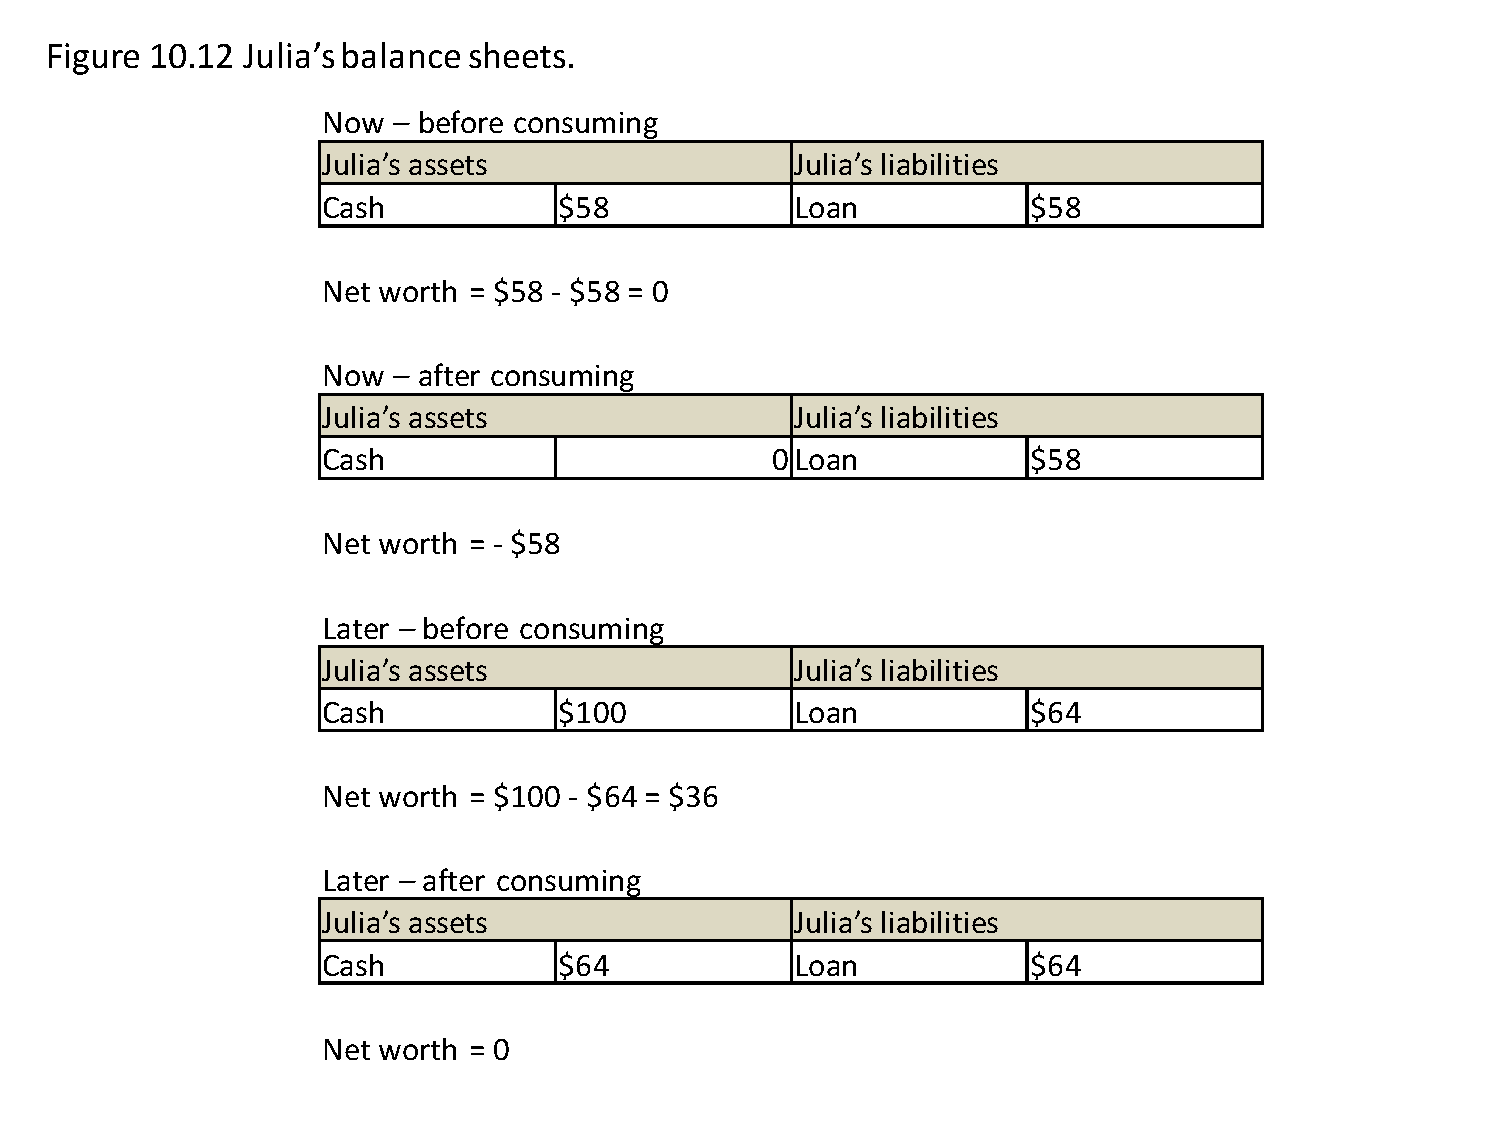
\includegraphics[trim={1.5cm 0.5cm 1.5cm 1.5cm}, clip, width=0.9\textwidth]{./figures/Figure14.pdf}
            \end{figure}
        \end{column}
    \end{columns}


\end{frame}

\begin{frame}{Banks}
\label{slide:Banks}
    \begin{itemize}
        \item Banks: firm that makes profits by lending and borrowing
        \item \alert{Borrow} from households (\textbf{deposits}), other banks, and the central bank at a \alert{lower} interest rate
        \item \alert{Lend} out loans at a \alert{higher} interest rate
        \item \alert{Cost}:
        \begin{itemize}
            \item operational: the salaries of bank officers, branch rents
            \item interest costs: paying interest on their deposits and other borrowing
        \end{itemize}
        \item \alert{Revenue}: interest and repayment of loans
        \item \alert{Expected return}: The return on the loans, taking into account \textbf{the default risk}.
    \end{itemize}
\end{frame}

\begin{frame}{Bank's Balance Sheet}
\label{slide:Bank_s_Balance_Sheet}
    \begin{figure}
        \centering
        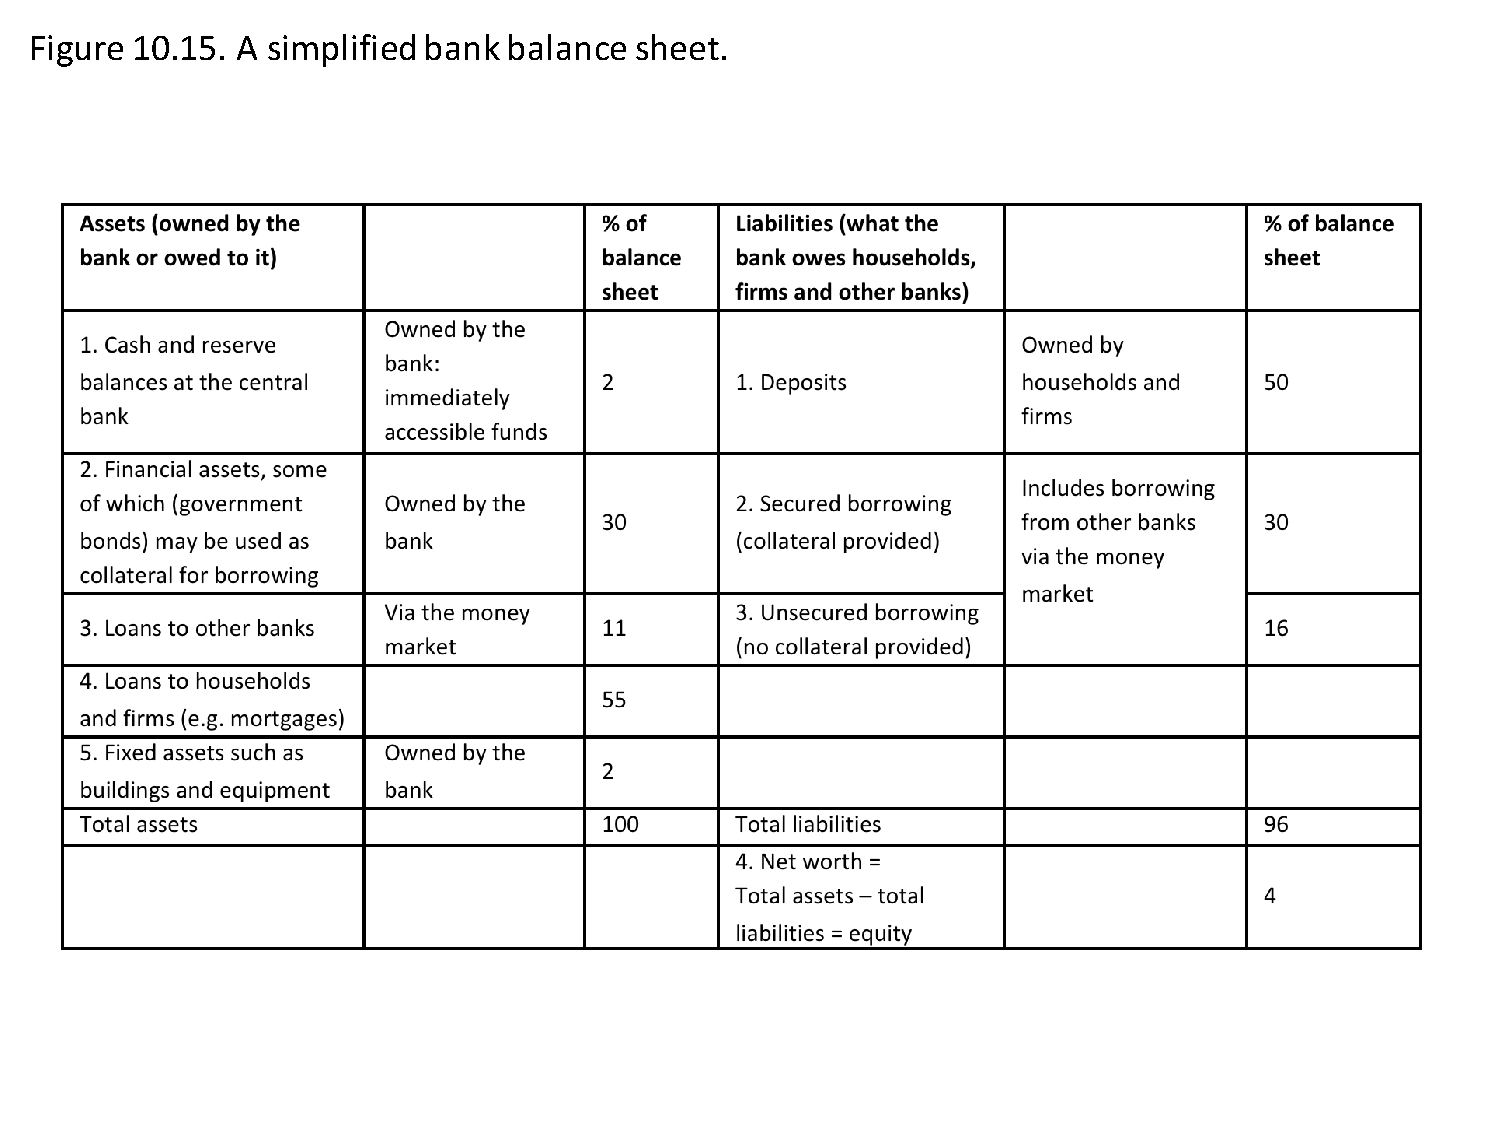
\includegraphics[trim = {0cm 0cm 0cm 1.5cm}, clip, width=\textwidth]{./figures/Figure22.pdf}
    \end{figure}

\end{frame}

\begin{frame}{Bank's Net Worth}
\label{slide:Bank_s_Net_Worth}
    \begin{center}
        Net worth = assets $ - $ liabilities
    \end{center}
    \begin{itemize}
        \item means what is owed to the shareholders/ owners
        \item also called \textbf{equity}
        \item net worth $ < 0$ means bank is \textbf{insolvent}
        \begin{itemize}
            \item i.e., unable to repay debt
        \end{itemize}
        \item Leverage describes the reliance of a company on debt:
        %
        \begin{equation*}
            \text{leverage} = \frac{\text{total assets}}{\text{net worth}}
        \end{equation*}
        %

    \end{itemize}

\end{frame}


\begin{frame}{Central Banks}
\label{slide:Central_Banks}
    \begin{itemize}
        \item \textbf{Legal tender} has to be accepted as payment by law
        \item \textbf{Base money/high-powered money}: notes and coins. Money as legal tender
        \item The central bank is the only bank that can \alert{create} legal tender.
        \begin{itemize}
            \item the central bank is usually owned by the government.
            \begin{itemize}
                \item Or not! e.g. \alert{Federal Reserve}
            \end{itemize}
            \item acts as the banker for the commercial banks, who have accounts at the central bank that hold legal tender.
            \item by crediting these accounts, the central bank can create money.
        \end{itemize}

    \end{itemize}

\end{frame}

\begin{frame}{Bank Money}
\label{slide:Bank_Money}
    \begin{center}
        \textit{Commercial banks create money by making loans}
    \end{center}
    \begin{itemize}
        \item this is called bank money $ \neq $ legal tender
        \item it is a liability to the bank, not an asset
        \item banks earn profits by charging interest on bank money
    \end{itemize}
    \begin{table}
        \newlength\pp
        \setlength\pp{\dimexpr .5\textwidth -2\tabcolsep}
        \begin{tabular}{p{\pp}|p{\pp}}
            Bonus Bank’s assets
                & Bonus Bank’s liabilities
            \\
            \hline
            \$20 base money
            \newline
            \$100 bank loan
            \newline
            Total: \$120
                & \$120 payable on
                \newline
                demand to Gino
            \\
        \end{tabular}
        \caption{Bonus Bank gives Gino a loan of \$100}
    \end{table}

    \begin{center}
        Broad money $ = $ base money $ + $ bank money
    \end{center}
\end{frame}

\begin{frame}{The Money Market}
\label{slide:The_Money_Market}
    \begin{itemize}
        \item Banks need enough base money to cover their net transactions.
        \item They borrow base money on the money market at the short-term interest rate.
        \begin{itemize}
            \item The demand for base money depends on how many transactions commercial banks have to make.
            \item The supply of base money is a decision by the central bank.
        \end{itemize}
    \end{itemize}
\end{frame}

\begin{frame}{Application: central bank's policy rate impact}
\label{slide:Application__central_bank_s_policy_rate_impact}
    \begin{columns}
        \begin{column}{0.3\textwidth}
            \begin{itemize}
                \item The central bank's policy rate affects the level of spending in the economy, because households and firms borrow to spend.
                \item \textbf{higher interest rate $ \rightarrow  $ low spending today}
            \end{itemize}
        \end{column}
        \begin{column}{0.7\textwidth}
            \begin{figure}
                \centering
                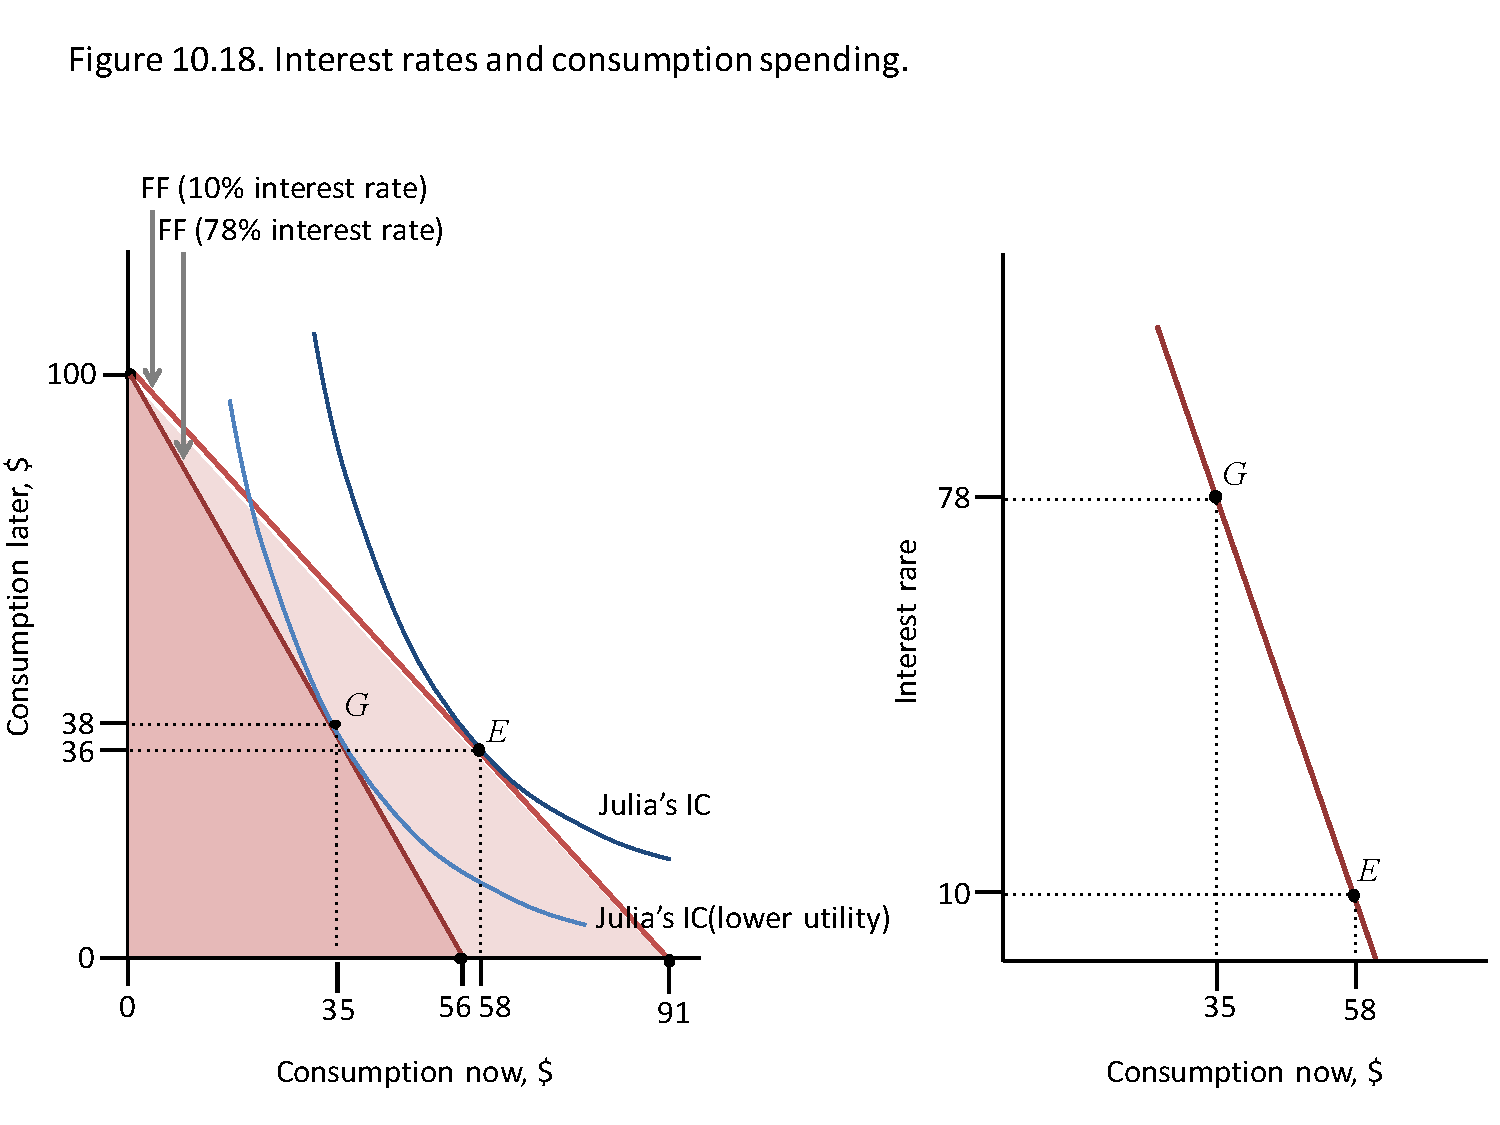
\includegraphics[trim = {0cm 0.5cm 0.5cm 1.5cm}, clip, width=\textwidth]{./figures/Figure25.pdf}
                \caption{Right: Credit market, Left: Loan Demand for Julia}
            \end{figure}

        \end{column}
    \end{columns}

\end{frame}

\section[ \faCreditCard \faLock ]{Credit Rationing}
\label{sec:Credit_Rationing}


\begin{frame}{Recall: Principal-agent Problem}
\label{slide:Recall__Principal_agent_Problem}
    \begin{itemize}
        \item Def: conflict of interest between principal (\alert{lender}) and agent (\alert{borrower})
        \begin{itemize}
            \item Lender has no info on borrower's effort in financial project $ \Rightarrow  $ loan may not repay
        \end{itemize}
        \item Resolution: \alert{equity constraint} and/or \alert{collateral constraint}
        \begin{itemize}
            \item Equity: require the borrower to put some of her wealth into the project
            \item Collateral: set aside property that will be transferred loan not repaid
        \end{itemize}
        \item Lender's risk $ \downarrow \downarrow  $, but at what cost?
    \end{itemize}

\end{frame}

\begin{frame}{Credit Rationing}
\label{slide:Credit_Rationing}
    \begin{itemize}
        \item Those with less wealth find it more difficult to provide equity or collateral
        \item \alert{Credit-constrained}: borrow on unfavourable terms compared with those with more wealth
        \item \alert{Credit-excluded}: refused loan entirely
    \end{itemize}

\end{frame}

\begin{frame}{Credit Rationing \& Inequality}
\label{slide:Credit_Rationing____Inequality}
    \begin{columns}
        \begin{column}{0.4\textwidth}
            \begin{itemize}
                \item Inequality may increase when some people are in a position to profit by \textbf{lending} money to others.
                \item Credit-rationing increases inequality: people with \alert{limited wealth} are \alert{not able to profit from the investment} opportunities that are open to those with more
assets.
            \end{itemize}
        \end{column}
        \begin{column}{0.6\textwidth}
            \begin{figure}
                \centering
                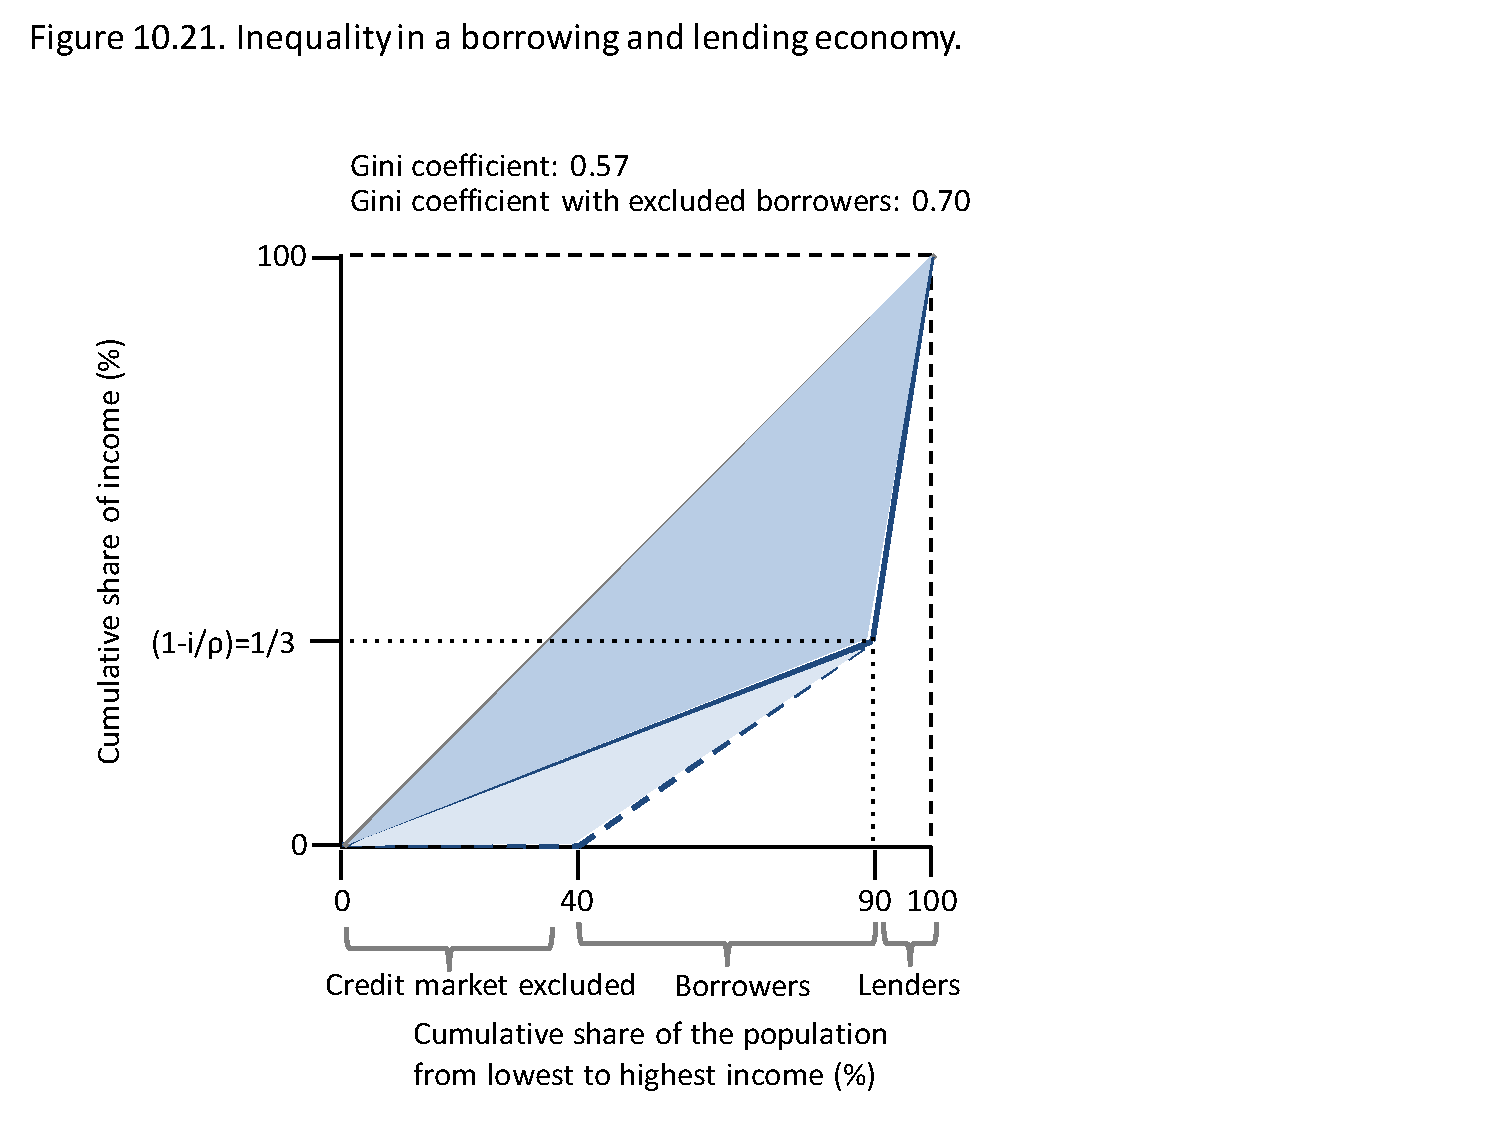
\includegraphics[trim = {1cm 0cm 8.5cm 2.5cm}, clip, width=\textwidth]{./figures/Figure28.pdf}
            \end{figure}

        \end{column}
    \end{columns}

\end{frame}


\end{document}
